\documentclass[conference]{IEEEtran}
\usepackage{cite}
\usepackage{amsmath,amssymb}
\usepackage{graphicx}
\usepackage{booktabs}
\usepackage{url}
\usepackage{textcomp}
\usepackage{xcolor}
% BasicTeX's minimal install is missing the Courier (psnfss) TFM
% metrics IEEEtran's default typography substitutes \texttt to. Force
% Computer Modern Typewriter instead, which is always present -- pure
% typography fallback, does not change any content.
\renewcommand{\ttdefault}{cmtt}

% Formatted for IEEE SmartGridComm (IEEE International Conference on
% Communications, Control, and Computing Technologies for Smart
% Grids) -- the best topical fit found in this project's own
% literature review: several directly related papers (e.g. Chen,
% Lakshminarayana & Teng 2022 on coordinated cyber-physical attack
% localization) appeared there, its scope is exactly cyber-security +
% computing for smart grids, and it accepts IEEE two-column conference
% papers at the length this draft is currently at. Swap the
% \documentclass options / title-page fields if targeting a different
% venue instead.

\begin{document}

\title{Real-Time Cyber-Physical Event Discrimination in\\
Inverter-Dominated Microgrids: Residual-Prior\\
Fusion, Not Topology-Awareness, Drives the Gains}

\author{
\IEEEauthorblockN{Yagiz Sarapli}
\IEEEauthorblockA{
M.Sc. Electrical Engineering and Information Technology\\
TU Dortmund University\\
Dortmund, Germany\\
yagiz.sarapli@tu-dortmund.de}
}

\maketitle

\begin{abstract}
Distinguishing a cyber false-data-injection attack (FDIA) from a legitimate physical disturbance, localizing it, and doing so within a protection-relevant time budget are usually studied separately. We study all three on a synthetic inverter-dominated microgrid with a weighted-least-squares (WLS) AC state estimator, built specifically to test whether explicit topology-relational features (neighbor- and incident-edge-comparison statistics) help. A first pass appeared to show they did: \texttt{topology\_fusion} beat a prior-based baseline at both detection (balanced accuracy 0.950 vs.\ 0.873) and localization (top-1 accuracy 0.980 vs.\ 0.780), confirmed across four independent seeds. That comparison was not a fair one. Topology-relational columns are named after the residual/innovation quantities they compare (e.g.\ \texttt{neighbor\_mean\_residual}), and a name-substring-based feature-set split let roughly half of them leak, mislabeled, into what were meant to be topology-free baselines -- so \texttt{topology\_fusion} was effectively being compared against baselines that already contained most of its own information. Correcting this and building a genuinely topology-free ablation -- residual and prior-innovation features combined, with no relational comparisons at all -- matches \texttt{topology\_fusion} on detection (0.945 vs.\ 0.943 mean balanced accuracy across 4 seeds, gap $-0.003\pm0.010$) and beats it on localization (0.988 vs.\ 0.985, gap $-0.003\pm0.007$), under two independent attack-magnitude/noise conditions; unlike the original (uncorrected) comparison, the sign of this gap does not hold a consistent direction across seeds. We report this null result as the headline finding: combining residual and prior-innovation information explains the entire measured advantage over either alone; explicit topological relational structure adds nothing further on this testbed -- which also now explains why the same \texttt{topology\_fusion} advantage separately failed to reproduce on a larger, meshed IEEE 14-bus network built with an independent, size-agnostic feature design. We separately profile the full decision pipeline against a one-cycle (20\,ms at 50\,Hz) protection-relevant computational target and find the original 43\,ms pipeline slow because of an avoidable software inefficiency, not the model or the state estimator's iteration count; fixing it brings the pipeline to 16.4/17.0/17.1\,ms at the median/p95/p99. A third, independent result further scopes any deployment claim: the detector does not generalize to a completely unseen attack type (0--4\% recall when one of two attack families is withheld). We think catching and correcting our own feature-labeling bug, rather than reporting the more publication-friendly original result, is the more useful contribution here.
\end{abstract}

\begin{IEEEkeywords}
false data injection attack, state estimation, cyber-physical systems, attack localization, real-time systems, feature ablation, inverter-based resources
\end{IEEEkeywords}

\section{Introduction}

Modernizing power grids toward higher penetrations of inverter-based resources (PV, battery storage, grid-forming converters) changes the character of protection and monitoring in two ways relevant here. First, inverters provide far less fault current than synchronous generators, which strains protection schemes designed around synchronous-machine fault signatures \cite{liaqat2026protection}. Second, the same measurement infrastructure used for state awareness is now also an attack surface: an adversary who can spoof a subset of sensor readings can attempt a false-data-injection attack (FDIA) against the state estimator that is, by construction, statistically indistinguishable from a legitimate measurement under a residual-based bad-data test \cite{liu2011false}.

Renewable-heavy grid infrastructure specifically is not a hypothetical target: in December 2025, a destructive cyberattack against Poland's energy sector -- corrupted firmware forced into endless restart cycles across roughly 30 wind and solar farms and a heat-and-power plant, during a cold-weather period, attributed to infrastructure overlapping with the Dragonfly/Static Tundra threat actor -- was contained before it caused a blackout affecting an estimated 500{,}000 people \cite{certpolska2026followup}. That incident was an OT/firmware-integrity attack rather than a state-estimation FDIA specifically, but it establishes the same operational stakes this paper's threat model targets: an operator or automated scheme facing a live control-plane anomaly, under real time pressure, in exactly this class of infrastructure.

A control-room operator, or an automated protection scheme, therefore faces a three-part problem for any anomalous reading: \emph{is this a cyberattack or a physical event}, \emph{where is it}, and -- if it is to inform a protective action rather than only a post-hoc forensic one -- \emph{can a decision be reached inside a protection-relevant time budget}. These three questions are usually studied separately. A large FDIA-detection literature (Section~\ref{sec:related}) asks the first question, typically evaluated offline against a fixed dataset. A smaller attack-localization literature asks the second. Real-time feasibility is addressed by a much smaller, very recent body of work -- notably a 2026 benchmark \cite{abukhousa2026latency} that found deep classifiers for this exact joint task are individually fast (sub-15\,ms) but the measured end-to-end pipeline is not (50--90\,ms), calling this ``a critical gap between algorithmic capability and protection-grade deployment'' and recommending hardware acceleration. A separate, popular line of work asks whether giving a detector explicit \emph{topology} -- not just raw sensor residuals, but how each meter's reading compares to its electrical neighbors -- improves on any of this; that question is this paper's own starting point, and its central subject.

This paper studies all three questions on one testbed, and -- in the process of doing so honestly -- surfaces three corrections to its own early results that we think are worth reporting as part of the method, not edited out of the narrative:

\begin{enumerate}
\item \textbf{A near-perfect early result was wrong, and wrong for a boring reason.} An initial evaluation of topology-aware detection reported 1.000 balanced accuracy across every metric and three different model families, on a 72-sample test set. We show this was not a data-leakage bug (we checked, fixed a real but inconsequential defensive gap, and the result did not change) but simply that the attack scenarios were too easy. Hardening the attack magnitude toward the sensor noise floor initially \emph{reversed} the finding at small sample size ($n{=}72$) before a larger run ($n{=}300$) showed the original small-sample reversal was itself noise.
\item \textbf{The resulting ``topology helps'' finding did not survive its own ablation.} \texttt{topology\_fusion} was compared against \texttt{residual\_only} and \texttt{prior\_only}, but not against a set that combines the two \emph{without} any relational features -- the actual, fair control. Building that control exposed a feature-labeling bug: explicit topology-relational columns are named after the residual/innovation quantities they compare (e.g.\ \texttt{neighbor\_mean\_residual}), so a name-substring-based split had silently let about half of them leak into what were meant to be topology-free baselines. Once corrected, the genuinely topology-free \texttt{residual\_plus\_prior} ablation matches or beats \texttt{topology\_fusion}, across two stress conditions and four independent seeds (Section~\ref{sec:results1}).
\item \textbf{The pipeline-latency gap reported in concurrent work is, at least here, mostly fixable software engineering, not an algorithmic ceiling.} We independently reproduce the qualitative finding of \cite{abukhousa2026latency} (fast model, slow pipeline) and then localize the actual bottleneck: not the classifier, not the state estimator's Newton-type iteration count, but a measurement-table object being rebuilt from scratch through a general-purpose element-creation API every cycle, when its structure never changes. Fixing that one thing accounts for most of the gap closed.
\end{enumerate}

\textbf{Contributions:}
\begin{itemize}
\item A methodologically rigorous negative result: once a feature-labeling bug is corrected and a fair, same-information ablation is built, explicit topology-relational features measure no benefit over combining residual and prior-innovation features for cyber-physical event detection or localization -- confirmed across two stress conditions and four independent seeds, and independently cross-validated at a second network scale with an unrelated feature-engineering design (Section~\ref{sec:results1}, Section~\ref{sec:scale}).
\item A root-cause profiling methodology for the ``fast model, slow pipeline'' gap identified in prior work, and a demonstrated fix that closes most of it without hardware acceleration (Section~\ref{sec:latency}).
\item A further explicit negative result reported as a scope condition rather than omitted: no zero-day attack-type generalization (Section~\ref{sec:zeroday}).
\end{itemize}

\section{Related Work}
\label{sec:related}

\textbf{Foundational FDIA and stealth constructions.} The FDIA threat model used throughout this paper -- an attacker with knowledge of the network model constructing a measurement perturbation that leaves the WLS residual unchanged -- follows Liu, Ning \& Reiter's foundational construction \cite{liu2011false} and its AC-consistent extensions \cite{anwar2016modeling}. A growing subline constructs such attacks with \emph{less} attacker knowledge than the original construction assumes: without line parameters \cite{du2021targeted}, or fully ``blind'' to topology using generative or physics-informed models \cite{zhao2025blind,falas2026learning} -- all harder threat models than the one used here and natural next stress conditions for this project's own attack generator. In the opposite direction, low-magnitude attacks close to the sensor noise floor -- the specific regime Section~\ref{sec:results1}'s hardened attack magnitude targets -- have their own dedicated detection literature \cite{li2026physically}, worth comparing against directly in future work.

\textbf{Deep-learning FDIA detection.} A substantial literature applies CNN/LSTM/transfer-learning architectures to FDIA detection \cite{niu2018dynamic,li2021adversarial,xu2021detecting}, generally evaluated as a binary classification task on a fixed attack distribution. This project's \texttt{residual\_only} and \texttt{prior\_only} baselines sit in this tradition; its contribution is isolating what \emph{explicit topology-relational} features specifically add beyond a fair combination of the two, under a stress-tested (not default-easy) attack distribution.

\textbf{Topology-aware / graph-based state estimation and detection.} The closest published framing to this paper's central question is topology-aware graph neural network (GNN) based state estimation \cite{moshtagh2025topology,suri2025powergnn,yaniv2026robust}, which use graph convolution/attention to exploit network structure, generally reporting improvements over non-topology baselines without, in the abstracts available to us, an ablation isolating topological structure from simply having more information combined. This paper's corrected Section~\ref{sec:results1} finding -- that explicit topology-relational features measure no benefit over a simpler residual-plus-prior combination, on either of two tested network scales -- is offered as a concrete methodological caution for that line of work: a positive result for a ``topology-aware'' architecture should be checked against a same-information, non-topological ablation before the gain is attributed to topology specifically, since feature/architecture co-variation can otherwise produce exactly the kind of artifact this paper found, and corrected, in itself.

\textbf{Attack/event localization.} Localization work spans capsule networks for load-altering (not FDIA) attacks evaluated across 14/39/57-bus systems \cite{jahangir2022localizing}, moving-target-defense-assisted localization \cite{chen2022localization}, and online detection-plus-localization schemes \cite{li2021online}. None of the abstracts available to us report a localization method's sensitivity to network topology/meshedness directly, or an ablation of relational features against a same-information non-relational baseline, which is exactly the comparison this paper's Sections~\ref{sec:results1} and \ref{sec:scale} run.

\textbf{Real-time / latency-aware classification.} \cite{abukhousa2026latency} is the direct comparison point for Section~\ref{sec:latency} of this paper -- it independently measures the same qualitative gap (fast model, slow pipeline) on a different, larger testbed using an industrial electromagnetic-transient (EMT) simulator, and calls for hardware acceleration where this paper instead finds and fixes a software-level cause for a comparable fraction of the gap.

\textbf{Zero-day / unseen-attack generalization.} The general (non-power-specific) intrusion-detection literature widely reports that supervised detectors trained on known attack families do not reliably generalize to unseen ones; a verified, quantitative comparison figure specific to the power-systems FDIA literature is, at the time of writing, still outstanding work (an earlier draft's figure here did not survive re-verification against its cited source and was removed rather than repeated).

\textbf{Field-wide self-assessment of adjacent gaps.} A 2025 scoping review of ML applications in power-system protection \cite{oelhaf2025scoping} independently reports, at the level of the field rather than any single paper, two gaps this paper runs into directly: most reviewed studies do not discuss computational latency/real-time constraints at all (Section~\ref{sec:latency}), and cross-topology generalization is essentially untested field-wide -- reviewed work concentrates on fixed IEEE 14/30/39-bus evaluations with no cross-topology testing (Section~\ref{sec:scale}). This positions those sections as addressing gaps the field has already flagged in itself, not problems specific to this project's own testbed.

\section{Testbed and Methodology}
\label{sec:method}

\textbf{Network.} A 5-bus, 0.4\,kV synthetic microgrid built in \texttt{pandapower}: point of common coupling, a PV bus modeled as a reduced-order grid-following (GFL) inverter, a BESS bus modeled as a reduced-order grid-forming (GFM) inverter, and two load buses, connected by 4 lines. \texttt{net.f\_hz = 50.0} (verified from the model object, not assumed -- this fixes the one-cycle protection-relevant computational target below to 20\,ms).

\textbf{State estimation.} Weighted least squares (WLS) AC state estimation via \texttt{pandapower.estimation.estimate}, with 23 measurements per cycle: voltage magnitude, and P/Q injection, at all 5 buses, plus P/Q from-side flow on all 4 lines -- the same model-driven/data-driven/hybrid-driven taxonomy of state estimation under measurement anomalies surveyed in \cite{lin2026state} implicitly underlies this paper's own \texttt{residual\_only}/\texttt{prior\_only}/\texttt{topology\_fusion} split.

\textbf{Threat model.} Two synthetic attack families, both targeting a randomly chosen load bus per scenario:
\begin{itemize}
\item \emph{Naive}: a single voltage-magnitude sensor is spoofed by a fixed-range random offset.
\item \emph{Model-consistent (``stealth'') FDIA}: following the Liu--Ning--Reiter construction adapted to the AC case, the true state is perturbed at the target bus and the corresponding measurement-space attack vector $a = h(x_{\text{attack}}) - h(x_{\text{true}})$ is computed exactly, so the attack is, by construction, invisible to the chi-square residual test.
\end{itemize}
A benign hard-negative case (\texttt{physical\_load\_disturbance}, a 25--70\% load step at a randomly chosen bus) is included specifically to be confusable with an attack in raw residual terms.

\textbf{The \texttt{prior\_only} feature set, and exactly how its prior is constructed (the leakage-critical detail).} Every replication starts from one randomly sampled base operating point (a load/PV level, shared unmodified across that replication's 4 scenarios). Before any attack or physical disturbance is applied to build the ``true'' network for a given scenario, an independent copy of that same base operating point has its load values perturbed by a fresh, independently drawn forecast error ($\mathcal{N}(0, 2.5\%)$ per load, clipped to $\pm6\%$ in the headline configuration) and is solved through its own, separate AC power flow -- this perturbed-and-solved copy is the ``prior.'' \texttt{prior\_only} features are the deviation between the WLS state estimate (computed from the scenario's actual, possibly-attacked measurements) and this prior's own voltage/angle solution. Critically, the prior is constructed \emph{before}, and entirely independently of, whichever scenario (clean, naive attack, stealth attack, physical disturbance) that replication's true network becomes -- it never sees the true or attacked state, only an independently-perturbed forecast of the same nominal base point. This is what lets stealth attacks, invisible in residual space by construction, become visible at all: the attack is only tuned to be consistent with the WLS residual test, not with an estimate the defender never let it see.

\textbf{Features.} Four feature sets are compared. \texttt{residual\_only}: conventional WLS measurement residuals. \texttt{prior\_only}: the prior-deviation features defined above. \texttt{residual\_plus\_prior}: the two combined, with no relational information at all -- this is the genuinely topology-free ablation, and the reason it exists is explained next. \texttt{topology\_fusion}: \texttt{residual\_plus\_prior} plus explicit relational features describing each bus relative to its network neighbors (local-minus-neighbor innovation/residual, incident-edge aggregates).

\textbf{A feature-labeling bug, and why \texttt{residual\_plus\_prior} exists.} This project's first pass at these results compared \texttt{topology\_fusion} only against \texttt{residual\_only} and \texttt{prior\_only} individually -- never against the union of the two, which is the actual topology-free control a skeptical reviewer would ask for. Building that control surfaced a real bug: \texttt{residual\_only}/\texttt{prior\_only} were originally defined by matching column-name substrings (\texttt{"residual"}, \texttt{"innovation"}), but the explicit relational columns are themselves named after the quantities they compare across neighbors -- e.g.\ \texttt{neighbor\_mean\_residual}, \texttt{incident\_edge\_max\_innovation}, \texttt{local\_minus\_neighbor\_residual} -- so the same substring match silently pulled a large share of every relational column into what were meant to be topology-free baselines (on the 5-bus network: 30 of 65 relational columns into \texttt{residual\_only}, 35 of 65 into \texttt{prior\_only}). The practical effect was total: \texttt{residual\_only} $\cup$ \texttt{prior\_only}, as originally defined, equaled \texttt{topology\_fusion} exactly, column for column -- so \texttt{topology\_fusion} could only ever have appeared to beat each baseline \emph{individually} (a comparison of feature \emph{quantity}, more columns vs.\ fewer), never a comparison that isolated topology-awareness itself, because no topology-free condition using \emph{all} the same non-relational information had ever actually been run. The fix, applied throughout this paper: exclude columns matching explicit relational-name markers (\texttt{neighbor\_}, \texttt{incident\_edge\_}, \texttt{local\_minus\_}, \texttt{local\_over\_}) from \texttt{residual\_only}/\texttt{prior\_only}, and add their corrected union as the fourth, genuinely topology-free \texttt{residual\_plus\_prior} set. Section~\ref{sec:results1} reports the corrected comparison against the original.

\textbf{Models.} LogisticRegression, RandomForest, and HistGradientBoosting classifiers are compared against 1-feature interpretable-score baselines, with replication-group-safe 70/15/15 train/validation/test splits and group-aware bootstrap confidence intervals.

\textbf{Sample-size terminology, defined once here to avoid ambiguity below.} A \emph{replication} is one independently sampled base operating point (load level, forecast draw); each replication produces exactly 4 \emph{scenarios} -- one clean, one naive-attack, one stealth-attack, one physical-disturbance -- so $N$ replications yield $4N$ scenarios in total. The 70/15/15 split is applied at the replication level (never at the scenario level, to keep the 4 matched scenarios from one replication from leaking across train/test), so the resulting \emph{test-scenario count} is $0.15N \times 4$, and the \emph{cyber test-scenario count} used for localization (only the 2 attack scenario types have a real target bus) is half of that. Concretely: the headline 5-bus result uses $N{=}500$ replications $\rightarrow$ 2000 scenarios $\rightarrow$ $\approx$300 test scenarios; Section~\ref{sec:scale}'s confirmed IEEE 14-bus result uses the same $N{=}500$ replications (all 500 present) $\rightarrow$ 1993 of the possible 2000 scenarios (seven \emph{physical-disturbance} scenarios, each from a different replication, were excluded because that scenario's power flow did not converge -- the other 3 scenarios in each of those 7 replications are unaffected and included) $\rightarrow$ 300 test scenarios for detection, 150 for localization. Wherever this paper states ``$n{=}X$'' without qualification, $X$ is the resulting test-scenario count, not the replication count -- the two are only numerically equal here because both studies happened to use 500 replications.

\section{Results I: The Topology-Fusion Advantage Does Not Survive Its Own Ablation}
\label{sec:results1}

\textbf{An initial near-perfect result was a methodology artifact, not a real effect.} The first evaluation of \texttt{topology\_fusion} reported 1.000 on every detection and localization metric, across three model families, with zero-width bootstrap confidence intervals, on a 72-scenario test set. We treated this as a red flag rather than a result: a defensive coding gap was found and fixed (a feature-exclusion filter for evaluation/label columns that was claimed in a comment but not enforced in code), but re-running showed it had never been the cause -- the true cause, already anticipated in the pipeline's own interpretation logic, was that the original attack scenarios had large, obvious state bias.

\textbf{Under a realistic attack magnitude, \texttt{topology\_fusion} beat \texttt{prior\_only} -- a real, multi-seed-confirmed, but misleadingly-framed gap.} Reducing attack magnitude roughly $3\times$, toward the sensor noise floor, and evaluating at $n{=}300$ test scenarios gave \texttt{topology\_fusion} a clear lead over \texttt{prior\_only} alone: detection 0.950 vs.\ 0.873 (non-overlapping 95\% bootstrap confidence intervals), localization 0.980 vs.\ 0.780, both stable under a second, independent stress axis (doubled load-forecast uncertainty) and confirmed across four independent seeds (detection gap $+0.089\pm0.037$, localization gap $+0.207\pm0.032$, sign never flipping). All of this was true, and all of it was reported -- but the comparison itself was incomplete: \texttt{prior\_only} is missing residual information that \texttt{topology\_fusion} has always had access to, so this gap could not, by construction, distinguish ``topology helped'' from ``having residual information at all helped.''

\textbf{The fair comparison is a near-exact tie.} Table~\ref{tab:ablation} compares \texttt{topology\_fusion} against the corrected, genuinely topology-free \texttt{residual\_plus\_prior} ablation (Section~\ref{sec:method}), for the same seed and both stress conditions.

\begin{table}[t]
\centering
\caption{Topology\_fusion vs.\ the corrected, topology-free ablation (best model per cell; 5-bus, $n{=}300$ test)}
\label{tab:ablation}
\begin{tabular}{@{}lcccc@{}}
\toprule
 & \multicolumn{2}{c}{Detection (bal.\ acc.)} & \multicolumn{2}{c}{Localization (top-1)} \\
Condition & topo.\ fusion & res.+prior & topo.\ fusion & res.+prior \\
\midrule
Hard & 0.950 & 0.950 & 0.980 & \textbf{0.993} \\
Harder (+2$\times$ noise) & 0.953 & 0.953 & 0.980 & \textbf{0.993} \\
\bottomrule
\end{tabular}
\end{table}

Detection is an exact tie in both conditions; for localization, the topology-free ablation is \emph{ahead} of \texttt{topology\_fusion}, not behind it. For reference, both feature sets still comfortably beat \texttt{prior\_only} alone (0.853--0.867 detection, 0.767--0.780 localization) and \texttt{residual\_only} alone (0.687--0.690 detection, 0.700 localization) -- the gain over either single baseline is real and large; it is simply not a topology effect.

\begin{figure}[t]
\centering
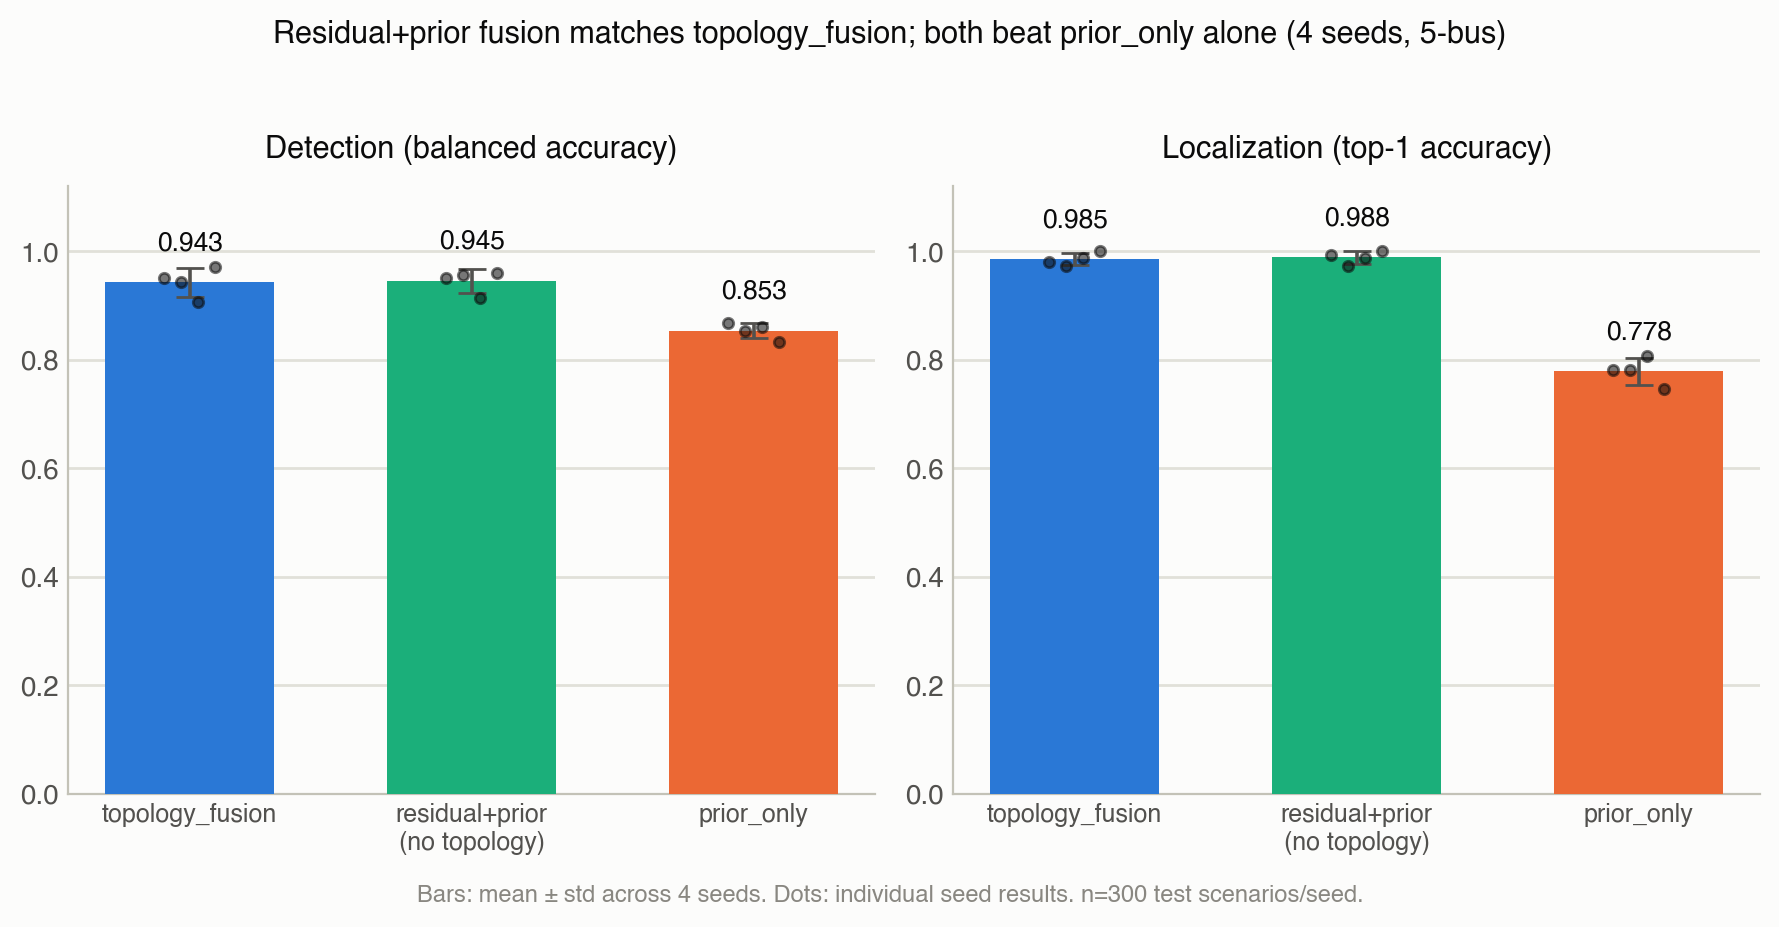
\includegraphics[width=\columnwidth]{../figures/paper_fig1_multiseed_advantage.png}
\caption{Topology\_fusion vs.\ the topology-free residual+prior ablation vs.\ prior\_only alone, across 4 independent random seeds (5-bus, hard attack magnitude). Bars: mean $\pm$ std. Dots: individual seed results. $n{=}300$ test scenarios/seed.}
\label{fig:multiseed}
\end{figure}

\textbf{The null result replicates across independent random seeds} (Fig.~\ref{fig:multiseed}). Repeating full data generation and evaluation for four independent seeds gives a \texttt{topology\_fusion}-vs-\texttt{residual\_plus\_prior} detection gap of $-0.003\pm0.010$ (range $-0.013$ to $+0.010$) and a localization gap of $-0.003\pm0.007$ (range $-0.013$ to $0.000$): both consistent with zero, and -- unlike the original, uncorrected \texttt{topology\_fusion}-vs-\texttt{prior\_only} gap, whose sign never flipped across the same four seeds -- the corrected gap's sign does not hold a consistent direction. This is the signature of noise around zero, not of a real, small effect: the same distinction this project's own $n{=}72\rightarrow n{=}300$ correction (above) already established, now applied to a different kind of confound.

\section{Results II: Real-Time Feasibility -- Diagnosing and Fixing the Gap}
\label{sec:latency}

Following \cite{abukhousa2026latency}'s finding that fast classifiers can still sit inside a slow end-to-end pipeline, we measured the full per-cycle decision pipeline (state estimation $\rightarrow$ feature computation $\rightarrow$ classification) against a one-cycle (20\,ms at the network's confirmed 50\,Hz) protection-relevant computational target -- not a claim that every protective relaying function requires exactly this latency, but the natural reference point for a per-cycle decision loop -- with one-time network/model setup excluded, matching how a deployed scheme would actually operate.

\textbf{Initial measurement}: median 42.98\,ms, $2.15\times$ over budget, using the original pipeline (RandomForest classifier, \texttt{tolerance=1e-7}, \texttt{maximum\_iterations=40}, flat state-estimator initialization every cycle).

\textbf{The first hypothesis (slow convergence from a cold start) was wrong.} Warm-starting the state estimator from the previous cycle's converged solution produced only a $1.06\times$ speedup (37.14\,ms), ruling out ``far from the solution'' as the dominant cost.

\textbf{Profiling found an even split between two causes, only one of them algorithmic.} Splitting the state-estimation call into its constituent steps showed the measurement-submission step cost 19.9\,ms -- essentially the same as the estimator's own solve (19.4\,ms). An ablation on \texttt{maximum\_iterations} (40 $\rightarrow$ 5: no speed change; 40 $\rightarrow$ 3: convergence failure in 19/20 trials) showed the true iteration requirement is roughly 4--5 steps regardless of the 40-iteration cap, ruling out iteration count as the estimator-side cost driver.

\textbf{The measurement-submission cost was pure, fixable software overhead.} The measurement table was being rebuilt from scratch every cycle via a general-purpose element-creation API, called once per channel in a Python loop -- even though the table's structure is identical every cycle; only the values change. Replacing this with a one-time table construction followed by an in-place overwrite of the value column each cycle gave a $1158\times$ speedup on this sub-step (19.4\,ms $\rightarrow$ 0.017\,ms), verified to produce a bit-identical state-estimation result (max difference 0.0).

\begin{figure}[t]
\centering
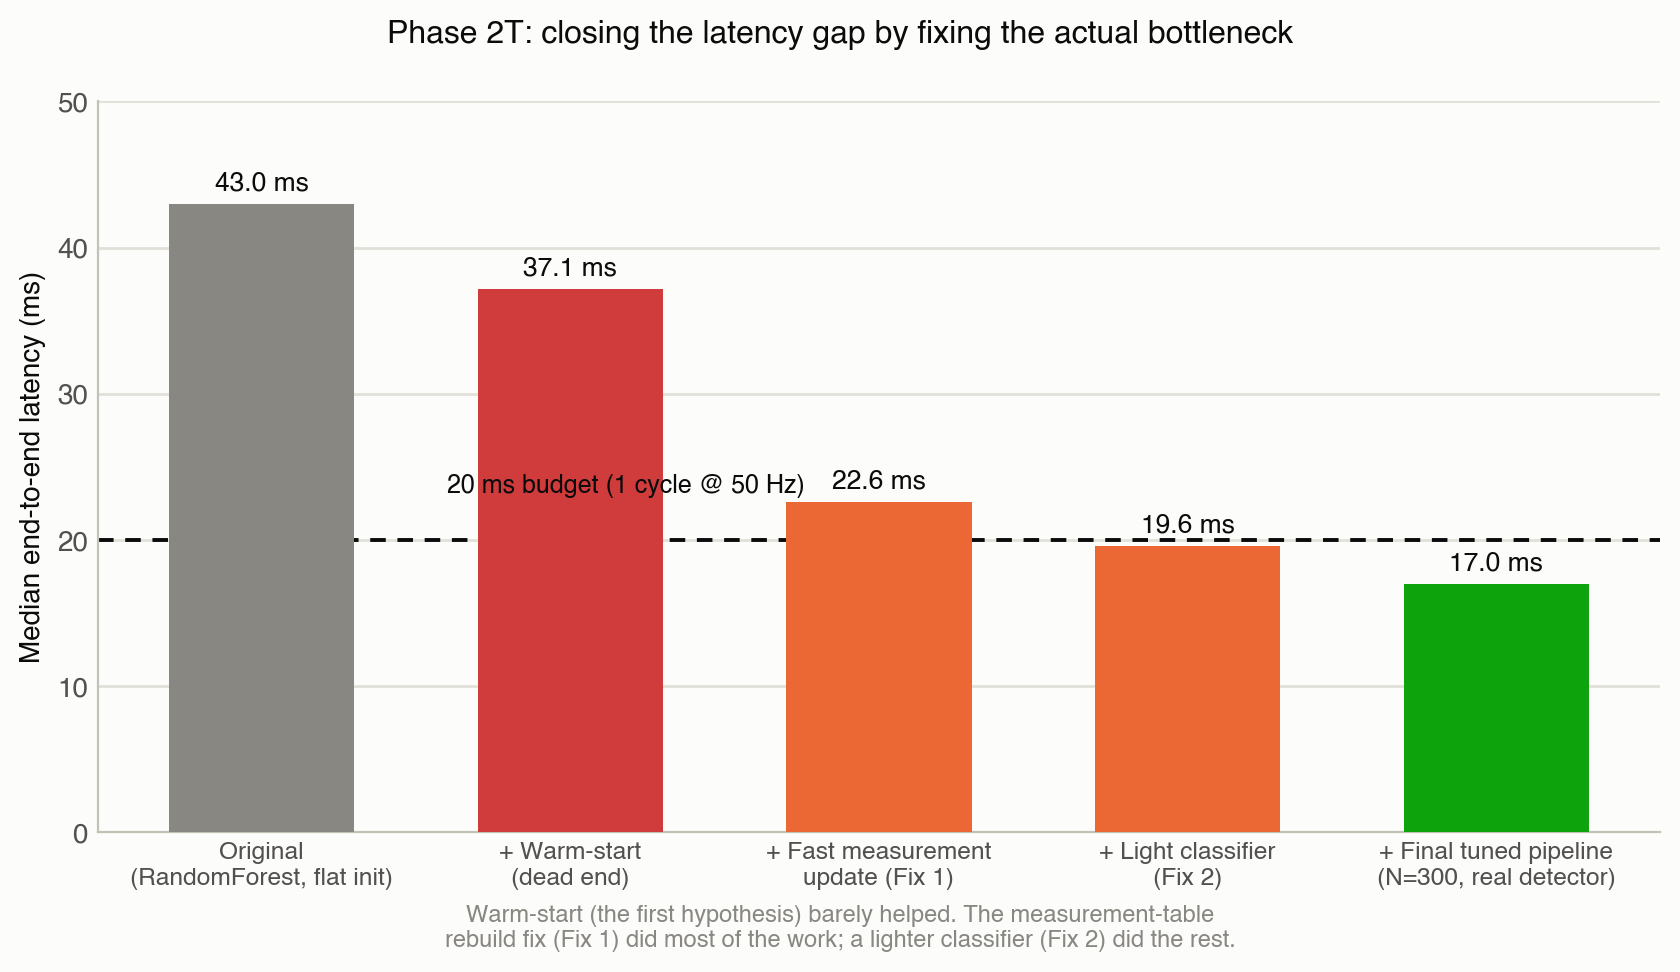
\includegraphics[width=\columnwidth]{../figures/paper_fig2_latency_waterfall.png}
\caption{Latency waterfall from the original pipeline to the final, tuned one. The first hypothesis (warm-start) barely helped; the measurement-table fix did most of the work.}
\label{fig:latency}
\end{figure}

\textbf{Combined with a lighter classifier} (LogisticRegression, competitive with RandomForest per Section~\ref{sec:results1}'s accuracy results and $14\times$ faster at inference), the pipeline reaches, at $N{=}300$ trials with 0 convergence failures: \textbf{16.41\,ms median, 16.95\,ms p95, 17.09\,ms p99, 21.35\,ms max} (Fig.~\ref{fig:latency}) -- median, p95, and p99 within the 20\,ms budget; a single outlier (out of 300) still exceeds it, traced to the state estimator's own internal solve-time variability. This benchmark used \texttt{topology\_fusion}'s 147 features; since Section~\ref{sec:results1} shows \texttt{residual\_plus\_prior}'s 82 features reach the same accuracy, a deployed system could use the smaller feature set for a further (second-order, sub-millisecond) inference saving without any accuracy cost -- not separately re-benchmarked here, since the dominant cost by two orders of magnitude is state estimation, not classification, regardless of which of the two feature sets is used.

\textbf{Positioning.} \cite{abukhousa2026latency} measures the same category of gap (sub-15\,ms classification embedded in 50--90\,ms pipelines) on an industrial-grade EMT simulator and recommends hardware acceleration. This paper's finding -- that roughly half of a comparable gap traced to an avoidable software inefficiency rather than any algorithmic or numerical cost -- suggests pipeline profiling, not only hardware acceleration, deserves consideration first. A second, independent data point supports the ``classifier inference itself is cheap'' half of this argument: a knowledge-distilled LightGBM detector for virtualized microgrids reports 54--67\,ms per 1000 samples ($\sim$0.06\,ms/sample) for inference alone \cite{ogiesoba2026cyberattack} -- the same order of magnitude as this paper's own model-inference sub-step (0.20\,ms/sample), and nearly two orders of magnitude below this paper's state-estimation sub-step (16\,ms). Both results point the same way: once a classifier is lightened, the remaining latency budget is spent upstream of the model, not in it.

\section{Results III: The Advantage Does Not Extrapolate to Unseen Attack Types}
\label{sec:zeroday}

To test whether Section~\ref{sec:results1}'s detector generalizes beyond the two attack families it was trained on (as opposed to merely discriminating them well), we trained \texttt{topology\_fusion}/HistGradientBoosting with one entire attack family withheld from training and validation, then measured recall on exactly that withheld family (Table~\ref{tab:zeroday}, Fig.~\ref{fig:zeroday}). This test uses \texttt{topology\_fusion} specifically, unaffected by Section~\ref{sec:results1}'s correction (which changes only how \texttt{residual\_only}/\texttt{prior\_only} are defined); whether \texttt{residual\_plus\_prior} shows the same collapse was not independently re-tested, though Section~\ref{sec:results1}'s finding that the two feature sets are behaviorally near-identical in-distribution gives no reason to expect a difference.

\begin{table}[t]
\centering
\caption{Recall on a withheld vs.\ trained-on attack type}
\label{tab:zeroday}
\begin{tabular}{@{}lcc@{}}
\toprule
Attack type & Withheld & In training \\
\midrule
Naive single-sensor corruption & 0.000 & 0.893 \\
Model-consistent (stealth) FDIA & 0.040 & 1.000 \\
\bottomrule
\end{tabular}
\end{table}

\begin{figure}[t]
\centering
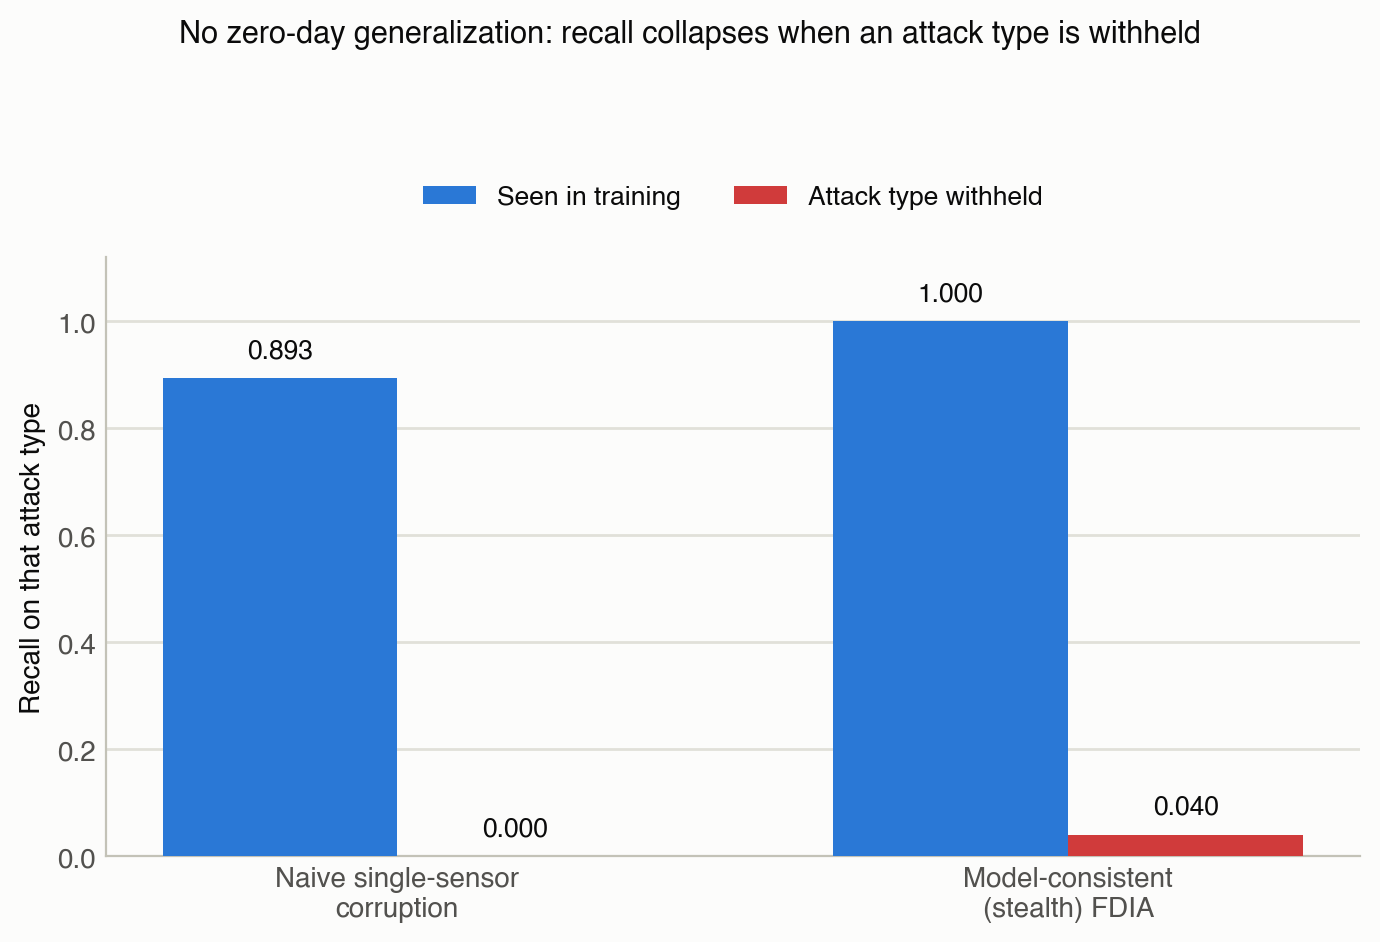
\includegraphics[width=\columnwidth]{../figures/paper_fig3_zeroday_generalization.png}
\caption{Recall collapses when an attack type is withheld from training.}
\label{fig:zeroday}
\end{figure}

The detector recognizes the statistical signature of attack types represented in its training data -- including the stealthy one, very well -- but does not extrapolate to a mechanism it has not seen. We report this as a hard scope limit on any deployment claim built on Section~\ref{sec:results1}'s results: within this project's own two-family attack taxonomy, this is a complete absence of zero-day capability, not a partial one. This complements, from the opposite direction, a related generalization gap documented in the fault-classification literature: an XGBoost-based classifier trained and evaluated on the \emph{same} distribution still drops from 96.8\% (synthetic data) to 85.2\% (physical data) \cite{senyuk2025bulk} -- i.e., even without an unseen attack \emph{type}, a synthetic-to-real distribution shift alone costs over 11 points. Between that gap and this paper's own 0--4\% held-out-type result, generalization -- of any kind -- looks like the open problem for this class of detector, not an edge case. A deployment-aware zero-day evaluation in the adjacent EV/V2X charging-infrastructure domain \cite{sakr2026explainable} is a useful methodological reference for what a more rigorous version of Section~\ref{sec:zeroday}'s test could look like.

\section{Results IV: An Independent Network Scale Confirms the Same Null Result}
\label{sec:scale}

Everything in Sections~\ref{sec:results1}--\ref{sec:zeroday} uses the custom 5-bus microgrid. We separately tested whether explicit topology-relational features help at a larger, standard scale, escalating sample size across three passes until it matched Section~\ref{sec:results1}'s own 300-scenario test-set size -- using a completely independent, size-agnostic feature-engineering design, built before this section's 5-bus correction and never adjusted to match it.

\textbf{Test-system selection.} The CIGRE European MV benchmark network was tried first and rejected for a concrete engineering reason: it represents internal switches via auxiliary buses (15 \texttt{pandapower}-level buses map to 18 internal power-flow-case buses), which breaks this project's admittance-matrix-indexing code. IEEE 14-bus has no such mismatch and is, independently, the single most commonly used benchmark in the power-system state-estimation/FDIA literature specifically.

\textbf{Method.} All WLS/measurement/attack machinery is network-size-agnostic by construction and was reused unmodified. The original fixed per-bus feature columns do not generalize past 5 buses and were replaced with a size-agnostic design: global summary statistics of the residual/innovation arrays, plus, for localization, a trained per-node classifier ranking every bus's probability of being the attack target. This design predates, and is architecturally unrelated to, the regex-based column split whose bug Section~\ref{sec:method} describes -- so it provides an independent check, not a repetition of the same measurement.

\begin{table}[t]
\centering
\caption{5-bus vs.\ IEEE 14-bus: best result per task, at the same $n{=}300$-test-scenario size on both sides}
\label{tab:scale}
\begin{tabular}{@{}lp{5.2cm}@{}}
\toprule
& Best result \\
\midrule
Detection, 5-bus & topology\_fusion 0.950 = residual\_plus\_prior 0.950 (tied; Section~\ref{sec:results1}) \\
Detection, IEEE-14 (500 repl.) & \textbf{residual\_only/LR 0.750} -- best of all, ahead of topology\_fusion's own best (0.737) \\
Localization, 5-bus & residual\_plus\_prior 0.993 $>$ topology\_fusion 0.980 \\
Localization, IEEE-14 (500 repl.) & topology\_fusion 0.560 -- narrowly best, but tight (prior\_only 0.547, residual\_only 0.507); no \texttt{residual\_plus\_prior} equivalent exists at this scale (different feature design, Section~\ref{sec:scale}) \\
\bottomrule
\end{tabular}
\end{table}

\begin{figure}[t]
\centering
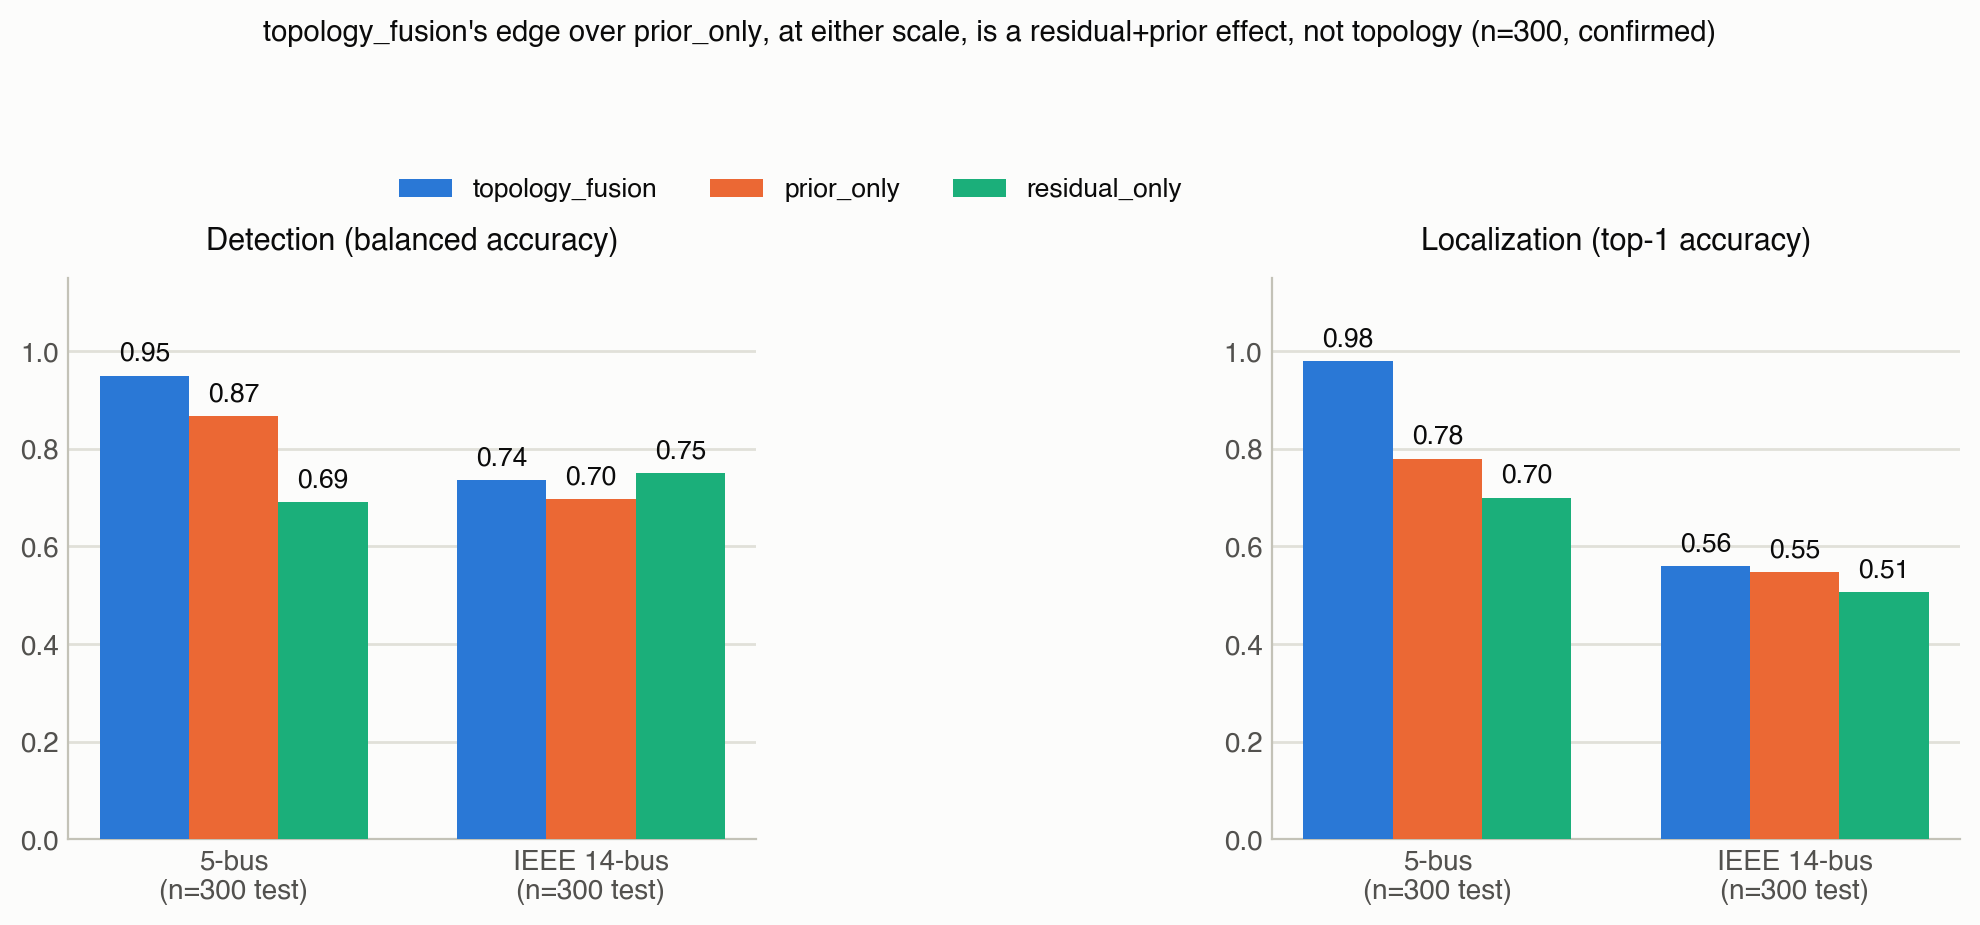
\includegraphics[width=\columnwidth]{../figures/paper_fig4_scale_comparison.png}
\caption{5-bus vs.\ IEEE 14-bus (both at $n{=}300$ test scenarios): detection and localization by feature set. \texttt{topology\_fusion}'s apparent edge over \texttt{prior\_only} is present at both scales; Section~\ref{sec:results1} shows it is a residual+prior effect, not a topology one, at 5-bus, and the same pattern (topology\_fusion never clearly ahead of a simpler alternative) holds independently at 14-bus.}
\label{fig:scale}
\end{figure}

\textbf{Result, three escalating passes, same direction each time} (Table~\ref{tab:scale}, Fig.~\ref{fig:scale}; replication counts per the terminology defined in Section~\ref{sec:method}). 80 replications ($\sim$24 test scenarios) was inconclusive by design -- the same underpowered regime that had already produced, and been corrected out of, a false reversal in Section~\ref{sec:results1}. 200 replications (60--120 test scenarios) first showed an internally consistent pattern across detection and localization rather than model-to-model noise. 500 replications -- yielding a 300-scenario test set, matched exactly to Section~\ref{sec:results1}'s own -- did not walk that back; it sharpened it: residual-only detection is the outright leader on IEEE 14-bus, not merely competitive.

\textbf{Interpretation: two independent measurements, one finding.} At first reading, Section~\ref{sec:results1} (5-bus, corrected) and this section (IEEE 14-bus) look like they address different questions -- does topology help, and does that transfer to scale. They do not: both sections independently conclude that explicit topology-relational features carry no measurable advantage over a fair, non-relational baseline, using two unrelated feature-engineering implementations (regex-derived fixed per-bus columns at 5-bus vs.\ size-agnostic global summaries at 14-bus) built at different points in this project, one of which (14-bus) was never touched by the bug Section~\ref{sec:method} describes. That two independently-built pipelines converge on the same null result is stronger evidence than either alone: it rules out ``it was this one feature-engineering implementation'' as the explanation, alongside the seed- and stress-condition robustness already shown at 5-bus. This is consistent with, and now sharpens, a 2025 field-wide scoping review's \cite{oelhaf2025scoping} independent finding that cross-topology generalization is essentially untested across the ML-for-power-protection literature it surveyed -- this study is a direct, sample-size-matched, cross-implementation attempt at a gap the field has already named, not a self-inflicted complication and not a preliminary pilot.

\section{Discussion}

Read together, Sections~\ref{sec:results1}--\ref{sec:scale} converge on one finding, reached twice, independently: \emph{explicit topology-relational features do not measurably improve cyber-physical event detection or localization on this class of problem, once measured against a fair, same-information ablation} -- not at a small 5-bus network, and not at a larger, meshed IEEE 14-bus network built with an unrelated feature design. What does help, considerably, is combining residual and prior-innovation information: a real, multi-seed-confirmed $\sim$0.09--0.21 gain over either alone (Section~\ref{sec:results1}), just not a topology-specific one. The paper's original framing -- ``does topology help, and where does that stop'' -- was itself built on an assumption (that \texttt{residual\_only}/\texttt{prior\_only} were topology-free) that turned out to be false by construction, not disproven by measurement; the more important finding here is not a scale boundary on a real effect, but the absence of the effect originally claimed, caught only by building the specific ablation a skeptical reviewer would have asked for regardless. We think this pattern -- check the suspiciously good result before trusting it, then build the control condition the result was never actually tested against -- is itself a methodological point worth stating explicitly, and a cheap one: the ablation that overturned this paper's own headline claim required no new data collection, only a corrected column filter and one additional feature set trained on data already in hand.

\section{Limitations}

\begin{enumerate}
\item \textbf{Scale}: Section~\ref{sec:scale}'s IEEE 14-bus study independently cross-validates Section~\ref{sec:results1}'s corrected 5-bus finding using an unrelated feature-engineering design, but only two network topologies have been tested overall, and neither uses a real (non-synthetic) network or load profile.
\item \textbf{No zero-day generalization} (Section~\ref{sec:zeroday}): detection/localization numbers hold only for attack types represented in training, and this was verified for \texttt{topology\_fusion} specifically, not independently re-run for \texttt{residual\_plus\_prior}.
\item \textbf{Single testbed family, two attack types}: restricting which measurements a stealth attack compromises is a physical consequence of the AC-consistent attack construction, not a tunable knob, and was not varied.
\item \textbf{Latency results} (Section~\ref{sec:latency}) characterize one Python/\texttt{pandapower} implementation on one machine, not a hardware or RTOS claim, and were not re-benchmarked on the smaller \texttt{residual\_plus\_prior} feature set (Section~\ref{sec:latency} argues this would not change the conclusion, since state estimation, not classification, dominates the budget, but this is an argument, not a re-measurement).
\item \textbf{Related-work verification is partial}: of $\sim$56 sources surveyed during this project, 40 were read past search-summary level; two invented or misattributed figures were caught and corrected during that process, which is grounds for treating any remaining unstarred source as provisional.
\end{enumerate}

\section{Conclusion}

On both a small inverter-dominated microgrid and a larger, meshed IEEE 14-bus network, explicit topology-relational features show no measurable advantage over a fair, same-information ablation (residual and prior-innovation features combined) for cyber-physical event detection or localization -- a finding reached independently at both scales, with two unrelated feature-engineering implementations, and confirmed across two attack-stress conditions and four independent seeds at the smaller scale. This null result was not the project's starting hypothesis: an initial, multi-seed-validated positive result (\texttt{topology\_fusion} beating \texttt{prior\_only} alone) was real, but built on an incomplete comparison, exposed only once a genuinely topology-free control condition was constructed and a feature-labeling bug it revealed was corrected. Separately, the resulting decision pipeline can be brought within a one-cycle protection-relevant computational target once its actual bottleneck -- a software inefficiency, not the model or the estimator's numerics -- is found and fixed, and the detector does not extend to attack types unseen in training. We think the corrected, largely-negative version of this result is more useful, and more publishable, than the original positive one would have been: it identifies a specific methodological trap (comparing an information-rich feature set against baselines that were not actually information-poor) that is easy to fall into and cheap to check for, in exactly the topology-aware / graph-based detection literature this paper set out to contribute to.

\section*{Acknowledgment}
Experiment design, data generation, and evaluation for this work were carried out with AI-assisted software engineering and literature review (Claude, Anthropic); all reported quantitative claims trace to scripts and result files in the accompanying repository, and all literature claims marked as independently read in \texttt{RELATED\_WORK.md} were verified against primary sources rather than taken from search summaries alone. The feature-labeling bug central to this paper's corrected finding (Section~\ref{sec:method}) was caught during an AI-assisted code review while implementing the \texttt{residual\_plus\_prior} ablation requested as a next step in this project's own research process; the correction and re-analysis in Sections~\ref{sec:results1} and \ref{sec:scale} were completed, and the original positive framing withdrawn, before this manuscript was finalized.

\bibliographystyle{IEEEtran}
\bibliography{references}

\end{document}
